\chapter{Essence Green Lighting}
\section{Abstract}

Many software engineering curriculum conclude with a
practicum or capstone project course. For courses involving external
clients, the course owner typically follows a Request for Proposal
process to vet (or green-light) qualified clients and projects.

Even though green-lighting projects does not guarantee project success, 
the goal is to reduce risks by systematically examining each proposal to identify
potential problems that the instructor could solve, mitigate against, 
or simply decide not to deal with by rejecting the proposal.

We propose and evaluate a Green-Lighting Approach based on the
SEMAT (Software Engineering Method and Theory) Essence framework. 
Our objective is to identify if such a framework could improve the Request for Proposal process 
at Carnegie Mellon University in Silicon Valley and other universities.

We conducted a case study by observing and interviewing the
course owner, examining a group of proposals, and identifying issues
with the current proposal process and practicum projects.
We proposed a green-lighting project state that, based upon Essence Alphas,
describes the minimal and ideal states that a project proposal should achieve to be accepted. 

The Green-Lighting Approach generated conversations among the faculty 
that clarified the guidelines for accepting and prioritizing proposals and identified deficiencies in our Request for Proposal. Additional work is required to refine the proposed Green-Lighting Approach based on current findings and further validate the approach.
  
Using Essence for green-lighting practicum projects in academia presents some limitations. 
The framework does not explicitly factor in business forces that affect proposal selection,
might be overly complex for the task, and might require modification with partial Alpha states. 
However, Essence provides a systematic approach for evaluating proposals based on various project dimensions. 
This approach could be used as an inspiration for deriving simpler custom green-lighting checklists. 

\section{Introduction}
\label{Introduction}

Many software engineering (SE) curricula finish with a practicum course
or capstone project \cite{GSWE}. At Carnegie Mellon
University in Silicon Valley, the curriculum culminates with a practicum
course in order for the students to demonstrate mastery of the
curriculum and to learn client management skills
\cite{Katz}. The practicum allows students to reinforce
their learning of core software engineering knowledge by applying this
knowledge to a different problem or domain. The practicum serves as
confirmation that the student has mastered the material. Earlier in the
curriculum, faculty manage the students project courses by playing the
customer or management role. The practicum provides an opportunity for
the students to work with a real client and practice client management
skills. Students actively manage the client engagement while faculty
observe and coach students without interfering unless necessary. The
students perform as a consulting team delivering a product that addresses the client's opportunity.

The university wants to increase its impact through the practicum
projects. The practicum course owner needs to find projects that
balance these goals:

\begin{itemize}
\itemsep1pt\parskip0pt\parsep0pt
\item
  maximize the students' learning experience, 
\item
  achieve a business goal or positively impact society, and
\item
  increase collaborations between university and industry. 
\end{itemize}

In order to accomplish the practicum goals, the faculty want to offer
a portfolio of projects including

\begin{itemize}
\itemsep1pt\parskip0pt\parsep0pt
\item
  a mix of project domains,
\item
  a mix of startups and established companies, and 
\item
  a mix of exploratory research and well defined
  endeavors.
\end{itemize}

Since we have a limited number of students and thus student teams, the
course owner needs to be selective about proposals with respect to these
goals. The course owner needs a systematic, non biased technique to
filter proposals.

\section{Related Work}
\label{Related Work}
Many software engineering professors have described their approach to providing a practical hands on experience. Most of the literature describes in detail how to run a team-based project course yet there is little discussion about the client selection process. 

In 1991, Shaw and Tomayko \cite{shaw1991models} examined hundreds of undergraduate software engineering courses and interviewed scores of instructors. In their technical report, they identify two major decisions that the instructor must make: 1) deciding the mixture of lecture and project components and 2) deciding the balance technical and managerial skills taught in the course. 

They describe several course models used in academia including the ``small group project'' model, ``large project team,'' model, and  ``the project only'' model. The ``small group project'' and  ``large project team'' models infuse lectures with a course long project. The ``project only'' model is typically a capstone course that focuses on the project experience.

Shaw and Tomayko discusses the importance of finding an interesting project that will motivate the students for the duration of the course, but provides no model for client selection.

In 2001, Cal Poly \cite {Turner2001} introduced a year long capstone project course. For the first two years, they relied on one industrial partner for the entire course, but due to coordination difficulties replaced the external project with a university project. No guidance is provided for project selection.

In 2002, Chamillard and Braun \cite{Chamillard2002} reflect on an undergraduate course at the U.S. Air Force Academy. They focus on tradeoffs such as the amount of guidance, documentation formats versus documentation examples, and focusing software development process versus product. They do not discuss their client selection process.

In 2002, Umphress, Hendrix, and Cross \cite{Umphress2002} reflect on their 18 years of experience and describe the transformation of processes from ad hoc, to MIL-STD-498 to IEEE 1074 to the Team Software Process to Extreme Programming. No information is provided about client selection.

In 2006, Coppit \cite{coppit2006} describes his strategies for overcoming the difficulties in running a large project team course including how to assess student performance. In his section on project selection, he briefly recommends that the amount of work should be commiserate with the length of the course, the scope needs to be flexible to allow cutting of features at the course's end, and have significant parallelizable work. 

In 2010, Ziv and Patil \cite {ziv2010capstone} discuss the experience of transitioning a capstone from one quarter to a three quarter course. The course follows a ``small group project'' model with external clients. The instructors typically have enough projects for all the enrolled students. Regarding selection criteria, the instructors take most projects within reasonable size, scope, goals and objectives, and reject only when the instructors notice a complete misunderstanding of the nature and purpose of a college-level undergraduate-level student project. 

Overall, criteria for client selection in the context of academic projects is only briefly discussed in the literature. 

\section{Background}
\label{Background}
For the past four semesters, we applied the Project Monitoring and
Steering Approach ~of the Essence framework
\cite{EssenceBook} in weekly Essence Reflection
Meetings \cite{EASE2014}. The approach provides student
teams with a simple, lightweight, non- prescriptive and method-agnostic
way to examine their projects holistically, structure team reflections,
manage risks, monitor progress and steer their projects
\cite{ICSE2014}.

During the research of applying the Project Monitoring and Steering
Approach, we observed practicum issues regarding stakeholder
representation, understanding the value of the opportunity, and undefined project scope and success criteria. Some aspects of these issues might be attributed to some extent to the way in which the practicum proposals are initiated and accepted. For example, one client believed that she could represent several different user personas and was unwilling for student teams to interview potential users. Our motivation is to examine our Request for Proposal process could help address these issues.

We proposed and applied a Green-Lighting Approach based on the Essence framework \cite{EssenceBook}. Our objective is to identify if such a framework could potentially improve the Request for Proposal process at Carnegie Mellon University in Silicon Valley and other universities.

The Green-lighting Approach
uses the Essence Alphas to describe how ready the project should be in
each Alpha, which we'll call ``green-lighting project state'' in this
paper. The green-lighting project state serves as a gating function,
filtering out unready projects.

In this paper, we will introduce the Green-lighting Approach which
provides a gating function for proposals. Section
\ref{Field Study Description} describes the field study
including the research goal, the current Request for Proposal, the
proposed change, and the study protocol. Section
\ref{Results} examines seven research questions
supporting the research goal. Section \ref{Conclusion}
summarizes that the findings and discusses future work.


\section{Green-lightning Approach of the Essence framework}
\label{Green-lightning Approach of the Essence framework}

In 2012, the SEMAT community released the Essence kernel
\cite{OMGStandard}. The Essence kernel describes a
software project through different dimensions called Alphas. For
example, the \textbf{Stakeholder} Alpha advances through the states
\textit{Recognized}, \textit{Represented}, \textit{Involved}, 
\textit{In Agreement}, \textit{Satisfied for Deployment}, and \textit{Satisfied in Use}. Each state has a set of checklist items. For example, \textit{Recognized} contains these three checklist items:

\begin{itemize}
\itemsep1pt\parskip0pt\parsep0pt
\item
  Possible stakeholders groups are identified
\item
  Team agrees on relevant stakeholder groups to be represented
\item
  Responsibilities of stakeholder representatives are defined
\end{itemize}

A project achieves a state when the team can check all the checklist
items for a state. This means that Essence represents projects through a
collection of linear state machines where the states are partially
ordered.

We defined the Green-lighting Approach based upon an example of using
the Essence framework from the Essence Book. Section 12: ``Running a
software endeavor: From idea to Product''
\cite{EssenceBook} describes how to use the Essence
Kernel Alpha States to define a staging process for a hypothetical
project. The example divides the project into four stages ``Getting
Ready to Start,'' ``Starting Up,'' ``Running Development,'' and
``Done.'' As the project progresses through these stages, the Alpha
states progress. In an organization managing many projects, one could
expect the projects to achieve certain states before making it into the
next stage. We define the Green-Lighting Approach to evaluate the
transitions between multiple stages.

The Green-Lighting Approach has three steps:

\begin{itemize}
\itemsep1pt\parskip0pt\parsep0pt
\item
  Evaluate each proposal and determine its state in each Alpha. For
  example, considering the  \textbf{Stakeholders} Alpha, a proposal that meets the three checklist items tor \textit{Recognized}
  and the four checklist items for \textit{Represented} would be marked as \textit{Represented} as seen in Figure
  \ref{EssenceAlpha}. This is repeated for each Alpha.
  This data can be represented as a hash where the keys are the Alphas
  and the values are the Alpha states, such as: \{stakeholders:
  ``represented'', opportunity: ``identified'', requirements:
  ``conceived'', software system: ``architecture selected''\}. The check marks in Figure
  \ref{EssenceAlpha} indicate the proposal's project
  state.
\item
  Determine the ``green-lighting project state,'' which is the minimal
  acceptable state for each Alpha. This too can be represented as a
  hash. In our example, the green-lighting project state could be:
  \{stakeholders: ``recognized'', opportunity: ``solution needed'',
  requirements: ``conceived'', software system: ``none''\}. The circled
  states in Figure \ref{EssenceAlpha} represent the
  green-lighting project state.
\item
  Applying the green-lighting project state to a proposal determines
  the project's readiness. A project is ready if the proposal has a
  larger or equal state for each Alpha in the green-lighting project
  state. Using the hash example, we compare each key of the hash and
  make sure the proposal is ``larger or equal'' to each corresponding
  key in the green-lighting project state. In the given example, the
  proposal is ready in each Alpha except Opportunity. In this regard, the approval process
  is a function with two inputs and one boolean output. F(Hash proposal,
  Hash greenlight\_project\_state) =\textgreater Boolean
  accept\_propopsal
\end{itemize}

% \begin{figure}[h]
% \includegraphics[scale=0.25]{EssenceAlpha.jpg}
% \caption{Essence alphas checked for a proposal and shaded for
% green-lighting project state}\label{EssenceAlpha}
% \end{figure}


\begin{figure}[!t]
\centering
\includegraphics[width=3.45in]{essence_green_lighting_images/EssenceAlpha.png}
\caption{Essence Alphas checked for a proposal and circled for
green-lighting project state}
\label{EssenceAlpha}
\end{figure}

In examining the seven Essence Alphas, only four Alphas,
\textbf{Stakeholders}, \textbf{Opportunity}, \textbf{Requirements}, and \textbf{Software System} are relevant to evaluating practicum proposals. The OMG standard defines these four Alphas as: \cite{OMGStandard}

\begin{itemize}
\itemsep1pt\parskip0pt\parsep0pt
\item
  \textbf{Stakeholders}: The people, groups, or organizations who affect or
  are affected by the software system.
\item
  \textbf{Opportunity}: The set of circumstances that makes it appropriate to
  develop or change a software system.
\item
  \textbf{Requirements}: What the software system should do to address the
  opportunity and satisfy the stakeholders
\item
  \textbf{Software System}: A system made up of software, hardware, and data
  that provides its primary value by the execution of the software.
\end{itemize}

The other three Essence Alphas (\textbf{Team, Way of Working} and \textbf{Work}) only make sense once a student team is
assigned to the project. Indeed, the \textbf{Team} has not been assembled yet,
hence it does not have a \textbf{Way of Working} and has not performed any
\textbf{Work}. By course design, the client does not determine the team's
\textbf{Way of Working}.


\section{Field Study Description}
\label{Field Study Description}

Following recommendations for reporting research done in the empirical
software engineering community
\cite{GQM, Shaw}, we formed our
research goal using Goal/Question/Metric:
\cite{GQM}

\begin{table}[h]
\renewcommand{\arraystretch}{1.3}
\centering
\begin{tabular}{|p{1.00in}|p{2.10in}|}
\hline
Analyze & SEMAT Essence’s Green-lighting Approach provided by the kernel Alphas and their states \\ \hline
for the purpose of & evaluation \\ \hline
with respect to its & effectiveness \\ \hline
from the point of view of the & educator and researcher \\ \hline
in the context of  & the software engineering practicum graduate course at Carnegie Mellon University. \\
\hline
\end{tabular}
\end{table}


This paper decomposes this goal into the following questions:


\begin{itemize}
\itemsep1pt\parskip0pt\parsep0pt
\item
  \textbf{Research Question 1}: What is the initial state of most projects
  based on the current proposals?
\item
  \textbf{Research Question 2}: What are some problems with the practicum that could potentially be mitigated to some extent prior to the start of the project?
\item
  \textbf{Research Question 3}: From the faculty perspective, what should be
  the minimum or ideal initial state of a project?
\item
  \textbf{Research Question 4}: How do the proposals compare against the
  proposed minimum and ideal green-lighting project states?
\item
  \textbf{Research Question 5}: Do we need to improve the Request for
  Proposal?
% \item
%   \textbf{Research Question 6}: What is the effect of using the Essence
%   Green-lighting Approach on the time it takes to accept or reject a
%   project?
\item
  \textbf{Research Question 6}: What are limits to the approach and
  limitations to its effectiveness?
\end{itemize}


\subsection{Current Practicum Request for Proposal}
\label{ProposalQuestions}

Prior to the start of the course, the course owner solicits project
proposals from industry and colleagues. The current practicum Request
for Proposal asks sponsors to create and provide a document including
the following information:

\begin{itemize}
\itemsep1pt\parskip0pt\parsep0pt
\item
  {Name of the project}
\item
  {Summary of the project}
\item
  {Overview of the sponsoring organization}
\item
  {Background and problem context }
\item
  {Relevance and Opportunity: why is it important and who benefits}
\item
  {Proposed scope of work}
\item
  {Major project goals and objectives }
\item
  {Technologies and skill sets requirements }
\item
  {Expected team size }
\item
  {Currently known obstacles}
\item
  {Nature of working relationship with sponsoring organization}
\item
  {Expected use of deliverables at project completion}
\item
  {Preliminary project roadmap}
\item
  {Criteria for measures of success}
\item
  {Any IP, NDA, or citizenship constraints}
\end{itemize}

The course owner wants any submitted proposal to clearly communicate
the project's big picture, the client's needs, and a general project
roadmap. At the due date, the course owner reviews the submitted
proposals to verify their completeness. The course owner verifies that
the project is an appropriate educational experience, and relies on the
students to filter the projects. The course owner encourages
students to contact the client for clarification, if necessary.

Given the number of students enrolled in the course, the course owner
determines the expected number of teams for the course. In years when
there are significantly more project proposals than expected number of
teams, the students use dot voting to cull the list down to a manageable
number. For example, for 32 students, there might be 6 to 8 teams. If
there are 16 acceptable proposals, the course owner reduces it to 12
practicum proposals by the students dot voting their favorite projects.

Once there is a ``shortlist'' of proposals, the course owner invites
all the clients and students to a practicum fair. The course owner asks
the students to be familiar with all of the practicum proposals. The
purpose is to provide a forum for the students to ask the clients
specific questions about the project, not for the client to give a
complete presentation about the project. The clients introduce themselves
and have a summary slide or two to remind the students about their
project. 

The students then submit a ranked ordering of all the projects from
their number one pick to their least favorite, and the course owner
forms teams. The course owner tries to assign students based upon their
first or second top choice while prioritizing paying clients. However,
this is not always possible when too many students select the same
project or when only one student selects a project.

\subsection{Proposed Practicum Request for Proposal}

We consider a modification to the current practicum Request for
Proposal process by adding a filtering step after the proposal are
received but before the proposals are shown to the students. For each
proposal, we evaluate the project's state described by the proposal
against a green-lighting project state defined using SEMAT Essence Alpha
states. The course owner only offers the students proposals that have
reached or exceeded the green-lighting state. If a proposal does not
meet the minimum criteria, then either the course owner rejects the
proposal or the course owner discusses issues with the sponsor to
illicit more information.

Various elements, like the university relationship with the client, or financial considerations, are not taken into account by the SEMAT Essence Kernel, which is the first identified limitation of the framework for the purpose of green-lighting projects in academia.

\subsection{Study Protocol}

The study protocol is as follows:

\begin{enumerate}
\itemsep1pt\parskip0pt\parsep0pt
\item
  We reviewed 21 submitted practicum proposals and
  identified their initial project state (refer to \textbf{Research Question
  1} for more information). In order to remove anchoring bias, we examined
  and rated each proposal independently. Any discrepancies were
  discussed in person.
\item
  Based upon our experience of observing the practicum course in the
  context of prior investigations \cite{EASE2014, ICSE2014},
  using a brainstorming session, we identified recent issues that
  might be addressable to some extent prior to the start of the course (refer to
  \textbf{Research Question 2} for more information).
\item
  During the same brainstorming session, we recommended a minimum and
  an ideal green-lighting project state, with the purpose of addressing
  the identified issues prior to the start of the course. The minimum
  and ideal states need to be realistic and feasible with respect to the
  kinds of projects that we receive (refer to \textbf{Research Question
  3} for more information).
\item
  We compared the state of 21 submitted proposals against the proposed
  minimum and ideal green-lighting project states (refer to \textbf{Research
  Question 4} for more information). Again, in order to remove
  anchoring bias, we reviewed and rated each proposal independently. Any
  discrepancies were discussed in person.
\item
  We proposed modifications to the current questions in the Request for
  Proposal to better reveal the initial green-lighting project state. We
  evaluated the new questions with the sponsors (refer to \textbf{Research
  Question 5} for more information).
\item
  We analyzed the study results and drew conclusions on the benefits
  and drawback of the proposed approach (refer to \textbf{Research Question 6
  } for more information).
\end{enumerate}

\section{Results and Discussion}
\label{Results}

\subsection{Research Question 1: What is the initial
state of most projects based on the current proposals?}

We started the Green-lighting Approach research by assessing the
initial states of the \textbf{Stakeholders}, \textbf{Opportunity},
\textbf{Requirements} and \textbf{Software System} Alphas for 21 proposals.

For the \textbf{Stakeholder} Alpha, we observed that:
\begin{itemize}
\itemsep1pt\parskip0pt\parsep0pt
\item
  33\% did not achieve any state. These proposals did not identify
  stakeholder groups.
\item
  48\% were in the \textit{Recognized} state. These proposals identified the
  stakeholder groups, but did not appoint the representatives.
\item
  19\% were in the \textit{Represented} state. These proposals
  identified the stakeholder groups and the representatives of each
  group.
\end{itemize}

For the \textbf{Opportunity} Alpha, we observed that:
\begin{itemize}
\itemsep1pt\parskip0pt\parsep0pt
\item
  53\% were in the \textit{Identified} state. These proposals indicated the
  need for a software solution with the stakeholders wishing to make an
  investment.
\item
  33\% were in the \textit{Solution Needed} state. These proposals clearly
  articulated the problem with confirmation on the need for a solution.
\item
  14\% were in the \textit{Value Established} state. These proposals
  established the business value with a clear definition of desired
  outcomes and success criteria.
\end{itemize}

For the \textbf{Requirements} Alpha, we observed that:
\begin{itemize}
\itemsep1pt\parskip0pt\parsep0pt
\item
  5\% did not achieve any state.
\item
  71\% were in the \textit{Conceived} state. These proposals captured the 
  itemize system purpose with the user types involved.
\item
  19\% were in the \textit{Bounded} state. These proposals defined their 
  scope with a clear definition of the success criteria.
\item
  5\% were in the \textit{Coherent} state. These proposals captured and
  prioritized the requirements.
\end{itemize}

For the \textbf{Software System} Alpha, we observed that:
\begin{itemize}
\itemsep1pt\parskip0pt\parsep0pt
\item
  90\% did not achieve any state. These proposals did not describe the
  platforms, technologies or languages for the project.
\item
  10\% were in the \textit{Initiated} state. These proposals identified the
  criteria for selecting the architecture. These proposals described the key technical risks and buy, build or reuse decisions made for the project.
\end{itemize}

\begin{figure}[!t]
\centering
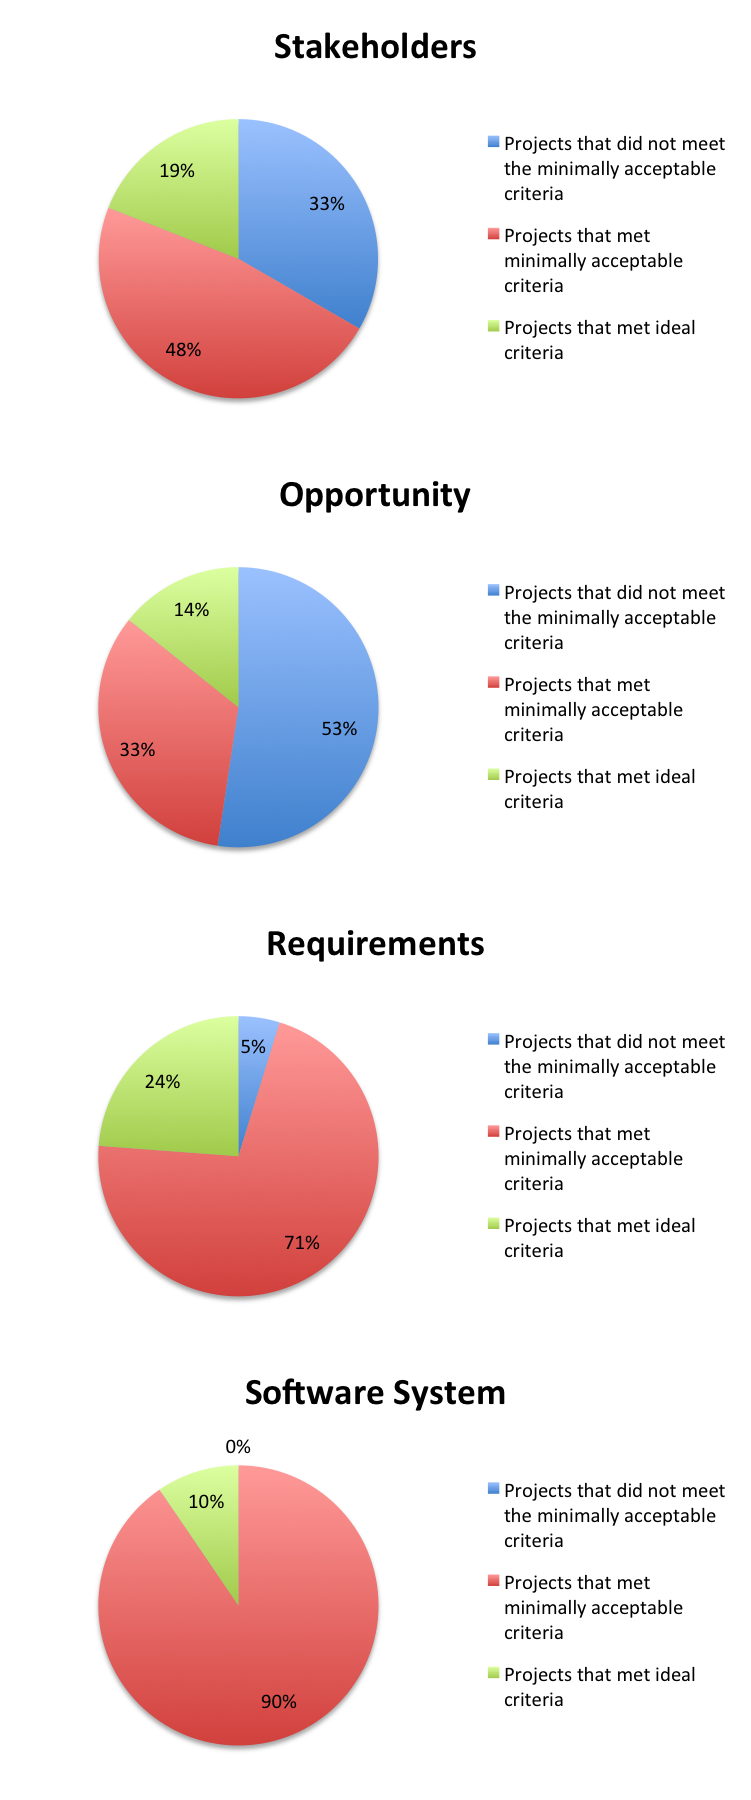
\includegraphics[width=3.45in]{essence_green_lighting_images/ProposalAlphasChartsStacked.png}
\caption{Essence Alphas checked for a proposal and circled for green-lighting project state}
\label{ProposalChart}
\end{figure}


In summary, we identified that 19\% of the proposals had represented
\textbf{Stakeholders}, 14\% of the proposals established the business value
of the \textbf{Opportunity}, 95\% \footnote{95\% is all the projects minus the 5\% that did not achieve any state} of the proposals captured the high level \textbf{Requirements} (and 24\% \footnote{24\% is the percentage of Bounded (19\%) and Coherent (5\%) projects} captured the project scope and success criteria), and 10\% of the proposals had defined criteria for selecting or identifying the \textbf{Software System} architecture. Since we do not expect the proposals to define architecture selection criteria, we are mostly concerned about the low
percentages for \textbf{Stakeholders} and \textbf{Opportunity} Alphas. Regarding
the \textbf{Requirements} Alpha, we would also like to increase the number of
proposals with defined project scope and success criteria.


\subsection{Research Question 2: What are some problems with the practicum that could potentially be mitigated to some extent prior to the start of the project?
}

While experimenting with Essence Reflection Meetings in the
context of practicum projects \cite{EASE2014, ICSE2014}, we
noticed that some practicum issues could potentially be identified and
addressed before the engagement started. These issues typically involve:

\begin{itemize}
\itemsep1pt\parskip0pt\parsep0pt
\item
  Missing stakeholder representation
\item
  Unclear opportunity value, and
\item
  Undefined project scope and success criteria
\end{itemize}

\textbf{Missing stakeholder representation:} Philosophical differences about
stakeholder representation present a challenge. The faculty believe that
most stakeholder groups should be represented and that a single
person cannot represent every stakeholder group because the groups
typically have very different needs. On one project, the team was building
a benchmark for comparing native code versus HTML5 code
on Android devices for the purpose of publishing the results to the
development community. While using the Essence framework for project
monitoring and steering \cite{ICSE2014}, the team
realized that no one represented the development community stakeholder
group. The team proactively interviewed local mobile developers and
presented the findings to the client. The client chose to ignore the
feedback putting at risk the potential benefit of the benchmarking
report to the development community. If a client is unwilling (or does
not understand the need) to have a representative for each (or most)
stakeholder groups, then the Request for Proposal process should
identify this issue and we can discuss our perspective with the client. If
the client is unwilling to change, we can decide to reject the
proposal.

\textbf{Unclear opportunity value and undefined project scope and success
criteria:} On a few projects, the teams spent the first two to three
weeks identifying the underlying problem and
analyzing the market trends and competitive landscape to validate the
need for a solution. Then they spent more iterations agreeing on the
project scope and success criteria. While this is an interesting
exercise, this significantly delayed the implementation work so the teams delivered substantially less functionality than the other
teams. Establishing the value of the opportunity and potentially
defining the project scope and success criteria at the start of the
practicum would have provided the practicum teams enough time to
build an interesting solution.

We believe that improving ``project readiness'' enhances the student experience, which remains to be verified in future research. If the stakeholder groups are not represented, then the
client can find representatives prior to the start of the project. If a client cannot clearly articulate the opportunity, the project's
benefits, the project's scope, or the project's success criteria, then
we can accept other proposals that have a larger impact.

Addressing these issues prior to the start of the practicum would
better align the expectations of the client with our educational goals, give the students a richer experience, provide more value to the client, and further the impact of the university.

\subsection{Research Question 3: From the faculty perspective, what should be the minimum or ideal initial state of a project?}

\begin{table*}
\renewcommand{\arraystretch}{1.3}
\caption{Green-lighting project state for each Essence Alpha (CMU1.1)}
\label{GreenLightingProjectState}
\begin{tabular}{|l|p{2.50in}|p{3.35in}|}
\hline
\textbf{Alpha}  & \textbf{Minimally acceptable}       & \textbf{Ideal}                        \\ \hline
Stakeholders    & \textbf{Recognized (Partial)}       & \textbf{Represented (Partial)}        \\ 
                & (check) Possible stakeholder groups are identified & (check) Stakeholder representatives are appointed \\
                & (not) Team agrees on relevant stakeholder groups & (check) Stakeholder representatives agree to take on responsibilities \\
                & to be represented                 & (not) Stakeholders agree on collaboration approach \\
                & (not) Responsibilities of stakeholder representatives  & (not) Representatives respect team's way of working \\
                & are defined                         & (check) Stakeholder representatives empowered to take on responsibilities \\ \hline
Opportunity     & \textbf{Solution Needed (Complete)} & \textbf{Value Established (Complete)} \\[5ex] \hline
Requirements    & \textbf{Conceived (Complete)}       & \textbf{Bounded (Partial)}            \\
                &                                     & (check) Purpose and extent of system are agreed \\
                &                                     & (check) Success criteria are clear \\
                &                                     & (not) Processes and tools for handling requirements are in place \\
                &                                     & (check) Scope constraints are identified \\
                &                                     & (not) Assumptions made while defining requirements are captured \\ \hline
Software System & None                                & \textbf{Architecture Selected (Partial)} \\
                &                                     & (check) Criteria for selecting architecture are agreed \\
                &                                     & (check) Platforms, technologies, languages are selected \\
                &                                     & (check) Selected architecture addresses key technical risks \\
                &                                     & (check) Buy, build, reuse decisions are made \\
                &                                     & (not) Stakeholders agree on necessary documentation \\
                &                                     & (not) Stakeholders agree on support service levels \\
                &                                     & (check) Non-functional architectural characteristics are considered \\ \hline
\end{tabular}
\end{table*}

After reviewing the practicum proposals and reflecting on practicum
issues listed in \textbf{Research Question 2}, we created green-lighting project
states for each Essence Alpha documented in Table~\ref{GreenLightingProjectState}.

The existing literature \cite{EssenceBook} implies
that staging (green-lighting in our case) can be done at the Alpha state level. In the process of creating our green-lighting project states, we discovered that for some of the Alpha states, we could not select all the checklist items in the entire state. For example, at the proposal stage, we do not expect responsibilities of the stakeholder representatives to be defined; this happens through a conversation between the team and the stakeholder representatives. In creating the green-lighting project state, we ignored some checklist items thus creating partial Alpha states.

The minimally acceptable and ideal states were defined with the goal of mitigating the problems identified in the previous research question, and based on the researchers expertise. Further work is necessary to validate the proposed states for each Alpha in the context of our practicum projects. Note however that other project courses might require different sets of minimally acceptable and ideal states to better address their specific needs.

\subsection{Research Question 4: How do the proposals
compare against the proposed minimum and ideal green-lighting project
states?}

Now that we have evaluated the proposals (Step 1) and created the
green-lighting project states (Step 2), we identify which proposals
meet the green-lighting criteria (Step 3 of the Green-lighting Approach). 

Table~\ref{table_proposal_evaluations} shows the proposals from the Spring 2014 and Summer 2014 semesters that meet the minimally acceptable and ideal criteria for green-lighting. 

\begin{table}
\renewcommand{\arraystretch}{1.3}
\caption{Proposals compared to green-lighting project states}
\label{table_proposal_evaluations}
\begin{tabular}{|p{1.10in}|p{0.95in}|p{0.95in}|}
\hline
Alpha & Number of projects that met minimally acceptable criteria & Number of projects that met ideal criteria \\ \hline
Stakeholders & 14 out of 21 & 4 out of 21 \\ \hline
Opportunity & 10 out of 21 & 3 out of 21 \\ \hline
Requirements & 20 out of 21 & 5 out of 21 \\ \hline
Software System & 21 out of 21 & 2 out of 21 \\ \hline
All (Satisfies all Alphas) & 8 out of 21 & 0 out of 21 \\ \hline
% Overall (Across all Alphas) & 8 out of 21 & 0 out of 21 \\ \hline
\end{tabular}
\end{table}

This analysis revealed a gap between the proposals and our
expectations, specifically in regard to representing stakeholders and
establishing the value of the opportunity. None of the proposals matched our ideal criteria across all Alphas, while 8 out of 21 satisfied our minimal expectation.

Around one third of the proposals did not have appropriate
representation for different stakeholder groups. In these proposals, the
client themselves would define, prioritize and validate the needs of the
different stakeholders groups. In our experience, when a team finishes
this kind of project, there is a high probability that the solution
would not deliver sufficient value for each stakeholders group. In some
cases, the solution may be unusable.

Around half of the proposals did not clearly state the
opportunity. The proposals described the problem to be solved, but did
not articulate the benefit of solving the problem. In a few cases, we
suspect the client has found a ``solution'' but has not yet identified
the problem to solve. In our experience, at the end of the project,
the project would be ``successful'' in delivering code to the client,
but might not solve a real world problem. Alternatively, the client
might have a detailed understanding of the opportunity, but may have not
clearly communicated that opportunity in the proposal.

The current proposals contain the same issues as the previous practicums identified in Research Question 2. The Green-Lighting Approach surfaced that the current proposals could repeat the problems identified in the past.


\subsection{Research Question 5: Do we need to
improve the Request for Proposal?}

In observing the gap between the proposals and our desired minimal
state, we wondered if asking different questions would help the sponsors
to record the kind of information that we need. Since the proposal's
content is a proxy for the sponsor's knowledge, is it possible that the
sponsor has more detailed knowledge that is not recorded in the proposal?
In addition, simply asking a question might cause the client to do some
groundwork not originally considered, which could potentially move the
project to a higher initial state. 

While analyzing the proposals, we had difficulty determining the stakeholder groups in the
 \textbf{Stakeholders} Alpha, the projected value of software system in the
 \textbf{Opportunity} Alpha, the list of high-level features that captures
the system purpose in the \textbf{Requirements} Alpha, and the non-functional
architectural characteristics in the \textbf{Software System} Alphas. The
Request for Proposal does not clearly ask for this information. We need
to ask specific questions to determine if the client can articulate the
answers. Improving the Request for Proposal would also facilitate
easier analysis for these aspects.

In order to help ascertain this information, we asked the sponsors four
questions.

{Survey Question 1. List your stakeholder groups and identify who will be
representing each group. (Note: Ideally there should be a different
person representing each group.)}

In examining the free-text answers, about \sfrac{2}{3} of the sponsors listed
out different stakeholder groups. A few even named who would fulfill the
role. One third of the sponsors listed themselves as the primary and
only stakeholder. In reviewing the proposals, these sponsors are not the
target stakeholder groups. This suggests that these proposals could be
misaligned with our educational goals of involving every stakeholder
group in the process.

{Survey Question 2. What value would the stakeholders receive from a successful engagement? If possible, please quantify the value (e.g. monetary
value, social return).}

In examining free-text answers, about half of the respondents were not
able to articulate the opportunity of the proposal. The other half of
the respondents appealed to social returns such as improving the
emergency response situations which could save lives and reduce injuries
or connecting seniors to their families and caregivers. None of the
respondents were able to put a monetary value to the opportunity.

{Survey Question 3. What features would you like to see implemented during the
practicum? }

In reviewing the free-text answers, about half of the sponsors provided
a feature list. The other half provided vague answers to the question.
This question needs to be rephrased. Perhaps asking the client to
prioritize the features to be delivered would be more effective.

{Survey Question 4. What are the key non-functional requirements (e.g.
scalability, security, performance, etc) that the solution should
satisfy?}

Most of the sponsors were able to clearly articulate the quality
attributes needed for the project. One sponsor said, ``Software will be
written in C/C++, documented well and reusable.'' 

When the answer does not fully or properly articulate the
non-functional requirements of the system, we recommend that the course
owner interviews the sponsor to acquire this information. 

The results from questions 1 and 2 are consistent with our assessment
of the proposals from Research Question 1. Adding these questions would
facilitate analysis but might not cause the sponsors to change the
stakeholder representation. Additional conversations between the course 
owner and the sponsor might be necessary.

Based upon these results, we plan to add questions 1, 2, and 4 to our
Request for Proposal. We will continue to experiment to find a question
that elicits a list of high-level features. These improvements to
our Request for Proposal will help us better assess the initial states
of the proposals.

% \subsection{Research Question 6: What is the effect of
% using the Essence Green-lighting Approach on the time it takes to accept
% or reject a project?}

% With modifications to the Request for Proposal questions, we believe
% that the Essence Green-lighting Approach would structure, simplify, and
% reduce the amount of time it takes to accept or reject a proposal when compared to our current process.
% However this remains to be verified.

In the current Request for Proposal process, the course owner reads
through each proposal to verify its completeness. We noticed that
clients submit ad-hoc proposals without necessarily following the
provided guidelines in terms of structure and content. This makes
assessing the readiness of each proposal arduous. The Request for
Proposal process provides a non-editable document and asks the sponsor
to address the items listed in Section
\ref{ProposalQuestions}. We recommend replacing this
document with a restructured editable template where the sections are
clearly aligned to the four Essence Alphas. Clients would be asked to
fill-in the sections of this template. 

% With the proposed Green-lighting Approach, the course owner still needs
% to read through each proposal, but instead of looking for completeness,
% the course owner assesses the four Essence Alphas in the green-lighting
% project state. This requires the small additional effort of reading
% through at most 23 checklist items, and even less if the proposals are
% less mature. These changes would reduce the time on task for the current
% verification for completeness of ad-hoc proposals by organizing the data
% provided by the client and simplifying the assessment of the
% green-lighting project states.

\subsection{Research Question 6: What are limits to
the approach and limitations to its effectiveness?}

\subsubsection{Green-lighting Approach does not factor important business considerations}
The approach provides data for a structured decision making process for
accepting and rejecting proposals, however, there might be reasons to
have a project go forward even though green-lighting says ``no.''
Several examples include paying clients, a high impact project, career
opportunity for students, and potential partnership for research
collaboration. While the approach provides a black and white answer,
we suspect that sound judgment is required for special circumstances.

\subsubsection{Green-lighting project states do not always
align to Alpha states}

In following the Green-lighting Approach, we discovered that partial
states, not Alpha states, represent our proposal acceptance criteria.
Some of the checklist items on one Alpha state would apply to accepting
a proposal and the rest of the checklist items would not. For example, 
for us to green-light a proposal, we would expect that the
proposal would meet the first checklist item of the
 \textbf{Stakeholders} \textit{Recognized} card, not the second or third as
described in Table \ref{GreenLightingProjectState}. 
Using partial states is possible but inconvenient. 

\subsubsection{Green-lighting Approach relies upon the Essence framework}
The Green-lighting Approach relies upon the Essence kernel for providing 
a systematic framework for evaluating proposals. The case study shows that  
only a subset of the framework is leveraged: Only 4 out of the 7 Alphas are 
relevant, and only the first few states (maximum 3) of each Alpha are necessary 
to green-light a project. In addition, some of the states need to be only partially 
considered as described in the previous section. Therefore, it is possible that a simpler checklist 
could be evolved, rather than relying upon the Essence framework. The extra 
complexity could be justified however if the project team continues to use 
the Essence framework during development to leverage mechanisms like progress 
monitoring and project steering. In that case it might make sense to use the 
same framework throughout the project.

\subsubsection{Green-lighting Approach does not guarantee project success}
Given the variety of issues that can emerge from a student project experience, and the fact that the initial state has only a limited impact on the overall project, the Green-Lighting Approach is not a silver bullet that will solve all team-based issues.
Only some risks might be reduced by systematically examining each proposal to identify
potential problems that the instructor could solve, mitigate against, 
or simply decide not to deal with by rejecting the proposal.

\subsection{Threats to Validity}
Internal Validity: This work assumes that it is desirable to filter
proposals and that is is possible to select proposals that will better achieve the
practicum goals listed in Section \ref{Introduction}. It could be the case
that a rejected proposal would have more significant learning
opportunities for the students than an accepted proposal.

Experimenter bias: We each had one years worth of experience in working with
the Essence framework prior to the start of this research. It is
possible that someone with less experience may encounter different results.

\section{Conclusions and Future Work}
\label{Conclusion}

This paper presents a first attempt to characterize and study a project 
selection process in academia. We proposed a Green-lighting Approach using the Essence framework and
applied the approach to the Request for Proposal process for the
practicum course at Carnegie Mellon University in Silicon Valley. 

After receiving and reviewing a set of proposals, the faculty determined each 
proposal state for each Essence Alpha. Based upon these initial states, prior experience, 
and recent problems, we created a gating function called green-lighting project
state to screen out proposals that are not ready for student teams.

After creating the green-lighting project state for each
Essence Alpha, we realized that our current Request for Proposal did
not prompt the clients to provide enough detail about the stakeholder
representations, the projected value of the opportunity, the project
scope and success criteria, and non-functional architectural
characteristics of the software system. We created draft 
questions and then tested the new questions with the prospective
clients. We recommend modifying our Request for Proposal to include
an editable template structured around the Essence Alphas and to include
several of the new questions identified in this paper. 

Further research is necessary to validate our green-lighting project state 
as well as our modified Request for Proposal. 
Even though green-lighting projects does not guarantee project success, 
the goal is to reduce risks by systematically examining each proposal to identify
potential problems that the instructor could solve, mitigate against, 
or simply decide not to deal with by rejecting the proposal.
More work is necessary to verify that our approach helps us reach that goal.

Using the Essence framework for green-lighting practicum projects in academia presents some limitations. 
First, the approach does not explicitly factor in business forces that affect proposal selection. 
Second, the Essence framework might be overly complex for green-light practicum projects, 
as only a subset of the Essence framework is necessary to perform the task.
In addition, the need to split the checklist items on the Alpha states to represent green-lighting 
project states prevents us from using the Essence cards out of the box hence losing the simplicity of the cards.

Still, project courses that use the Essence framework during development (to leverage mechanisms such as progress 
monitoring and project steering \cite{ICSE2014}) might want to borrow some ideas from the proposed Green-Lighting Approach, 
as it might make sense to leverage the same framework throughout the project.
In that case, we recommend customizing the approach by defining minimally acceptable and ideal states based on the course specific needs. 

For project courses that are not planning on using Essence during development, 
the framework could still be used as an inspiration for deriving simple custom green-lighting checklists for various project dimensions. Better aligning client proposals and educational goals has the potential of enhancing the students learning experience.
